\section{Chain-of-Steps 推理机制}

\subsection{CoF 与 CoS 的根本区别}

Chain-of-Frames (CoF) 假设视频推理沿帧顺序展开：第 1 帧提供线索，第 2 帧继承并推进，第 3 帧继续向后传递。这个直觉来自人类观看视频的方式，也来自语言模型中自回归生成的类比。

本文提出的 Chain-of-Steps (CoS) 则认为：视频扩散模型的推理主要沿 diffusion denoising steps 展开。在每个去噪步骤中，由于 DiT 对整段视频 token 做双向注意力，模型可以同时读取所有帧、所有位置的信息，进而全局更新整段视频 latent。于是推理不是“这一帧想完再轮到下一帧”，而是“每一轮去噪都把整段视频一起重写得更合理”。

\subsection{为什么可视化 $\hat{x}_0$ 能观察推理}

每个 diffusion step 的 $x_s$ 是当前带噪工作状态，不适合作为直接可视化对象。论文计算

\begin{equation}
    \hat{x}_0 = x_s - \sigma_s v_\theta(x_s,s,c)
\end{equation}

并解码它，相当于问：在当前 step，如果模型现在就停止生成，它认为最终视频应该是什么。把所有 step 的 $\hat{x}_0$ 排开，就可以观察语义决策如何从模糊、多候选逐渐收敛。

\subsection{Multi-Path Exploration}

多路径探索指早期扩散步骤中，模型会在 latent workspace 里同时保留多条可能解路径。这类似于搜索树或广度优先搜索：先展开多个候选，再逐渐剪枝。

Figure~\ref{fig:figure2} 中的多个例子展示了这种现象。机器人导航任务中，模型早期同时探索迷宫上方路径和下方路径，后续步骤逐渐压制一条路径并保留另一条。井字棋任务中，模型早期会同时标出多个可能获胜格子。物体移动任务中，模型会先提出多条潜在轨迹，对应不同货架层，最后收敛到正确放置位置。

\begin{figure}[H]
    \centering
    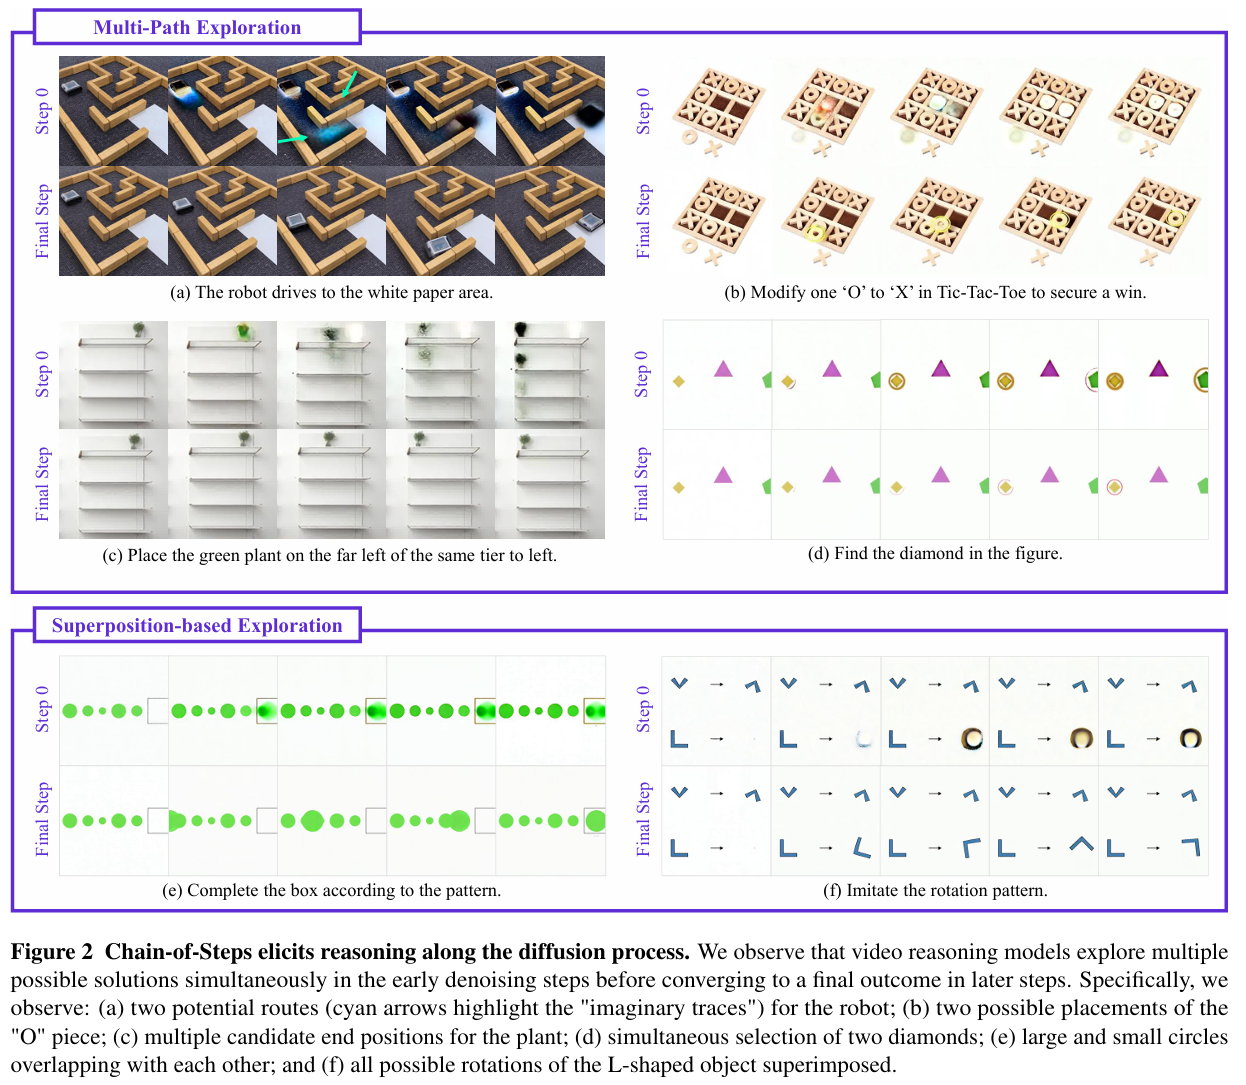
\includegraphics[width=0.96\textwidth]{figures/figure2.png}
    \caption{逐步推理的两种模式：多路径探索和基于叠加的探索。}
    \label{fig:figure2}
\end{figure}

这种行为与 LLM 中的 Tree of Thoughts 有相似性。CoT 是单链推理，而 ToT 显式生成多个 thought 分支、评估、剪枝并可能回溯。视频扩散模型并没有显式外部树搜索，但在 latent 空间中自然出现了类似多候选轨迹的结构。

\subsection{Superposition-Based Exploration}

基于叠加的探索指模型在早期步骤中同时表示多个互斥的逻辑状态，而不是立即选择一个。例如尺寸模式补全任务中，正确规律可能是“大-中-小”循环。模型早期会生成多个重叠大小的圆，表示对正确延续方式的竞争性假设。旋转任务中，模型可能先生成包含多个候选朝向的模糊表示，再逐步解析为单一角度。

多路径探索更像“多个空间路径并行存在”，而叠加式探索更像“同一位置上多个候选答案重叠存在”。二者都支持 CoS：早期 step 发散，中期 step 筛选，后期 step 定稿。

\subsection{Figure 1 的阶段解读}

Figure~\ref{fig:figure1} 中的迷宫示例可以分成三个阶段：

\begin{enumerate}
    \item Initial Attempt：早期 step 出现多个半透明候选路径，模型尚未确定最终路线。
    \item Pruning Paths：中期 step 中，不合理路径逐渐变弱，一条候选开始占优。
    \item Final Decision：后期 step 中，备选路径消失，只剩清晰最终路线。
\end{enumerate}

如果推理主要沿 frame 展开，我们会期待横向帧序列中逐帧推进的逻辑更明显。但图中最强的演化是纵向的：同一帧在不同 step 下从多解到单解。这是论文反驳 CoF、支持 CoS 的关键可视化证据。

\subsection{噪声扰动与信息传播}

论文进一步通过噪声注入验证 CoS。Figure~\ref{fig:figure3} 对比两种扰动：

\begin{itemize}
    \item Noise at Step：在某一个扩散步骤上，对所有帧注入高斯噪声。
    \item Noise at Frame：在某一特定帧上，在所有扩散步骤中持续注入高斯噪声。
\end{itemize}

\begin{figure}[H]
    \centering
    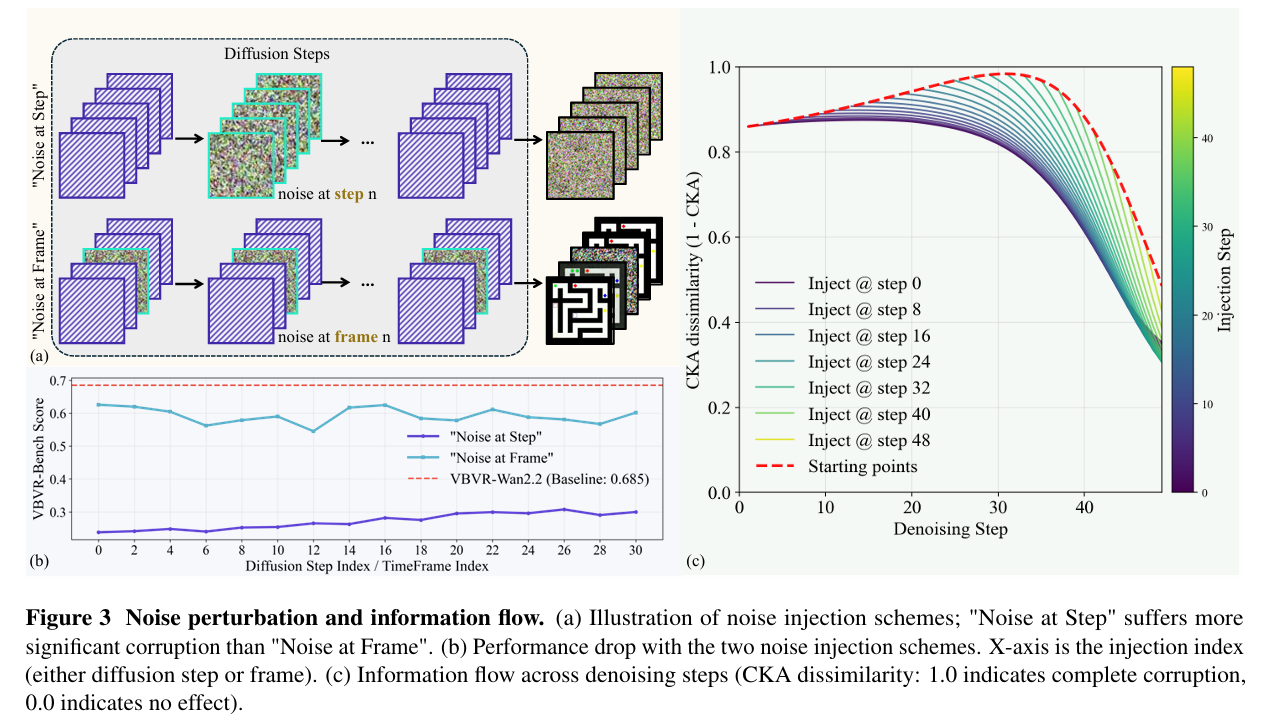
\includegraphics[width=0.96\textwidth]{figures/figure3.png}
    \caption{噪声扰动与信息传播分析：step-wise 扰动比 frame-wise 扰动破坏更大。}
    \label{fig:figure3}
\end{figure}

实验发现，step-wise 噪声会显著降低最终性能，而 frame-wise 噪声影响较弱。这说明关键推理状态更依赖扩散步骤，而不是单个帧。原因是每个 step 中模型通过双向注意力联合处理整段视频，被破坏的一帧可能在后续 step 中借助其他帧恢复；但如果某个关键 step 的全局 latent 被破坏，后续轨迹会整体偏移。

\subsection{中间步骤最关键}

论文还使用 CKA dissimilarity 分析扰动传播。结果显示，早期扰动会沿后续扩散轨迹传播，且敏感性在中间步骤达到峰值。原始笔记中记录敏感区约在第 20--30 步。

这与可视化观察一致：早期 step 还在探索，中期 step 正在剪枝并巩固主要结论，因此中期被破坏会造成最大影响。更后期 step 主要补细节，改变最终推理结论的能力反而较弱。
